\documentclass{article}
\usepackage[dblblindworkshop]{neurips_2026}
\workshoptitle{Managing Agents that Manage Agents}
\usepackage[T1]{fontenc}
\usepackage[utf8]{inputenc}
\usepackage{microtype}
\usepackage{amsmath,amssymb,amsthm,mathtools}
\usepackage{booktabs,tabularx,array}
\usepackage{enumitem}
\usepackage{xcolor}
\usepackage{hyperref}
\usepackage[nameinlink,capitalize]{cleveref}
\usepackage{natbib}
\usepackage{tikz}
\usetikzlibrary{arrows.meta,positioning,fit,shapes.misc}
\newtheorem{definition}{Definition}
\newtheorem{theorem}{Theorem}
\newtheorem{proposition}{Proposition}
\newcommand{\Reach}{\operatorname{Reach}}
\newcommand{\Acc}{\operatorname{Acc}}
\newcommand{\llbracket}{[\![}
\newcommand{\rrbracket}{]\!]}
\definecolor{accent}{RGB}{140,28,38}
\hypersetup{colorlinks=true,linkcolor=accent,citecolor=accent,urlcolor=accent}
\setlist{nosep,leftmargin=*}

\title{Contracted Hierarchies for Long-Horizon Meta-Agent Management}
\author{Anonymous Authors}
\date{}
\begin{document}
\maketitle
\begin{abstract}
Researchers and developers increasingly compose persistent chat, research, and coding-agent surfaces into informal long-horizon workflows, while retaining most coordination in human attention. We present a package-resident meta-agent management protocol that formalizes this pattern. Main is a persistent planning and decision chat; Theory and Experiment are optional specialist reasoning workstreams; Main authors one durable multi-view intent contract (DIC) and the initial execution prompt stack (EPS) for each approved Phase; a repository-aware coding-agent Orchestrator validates and model-tunes that prompt graph for the active surface, executes bounded Workers/subagents, and may issue contract-preserving repair EPS revisions. The DIC also acts as a human-intelligibility interface that preserves one Primary Aim and prioritized requests while hiding routine execution noise. Verification returns accept, repair, replan, or material escalation. Under complete read/write declarations and versioned evidence, a repair need invalidate only its dynamic dependency cone, and that cone is worst-case tight; we also bound fault survival under imperfect verification and characterize a checkpoint-cost trade-off. We introduce human-attention intensity---supervisory attention per unit of verified progress---as an evaluation target rather than an established performance result. The reference implementation provides reconstructable lineage and model-tuned execution controls, while a frozen matched-budget study is designed to test whether the hierarchy improves trustworthy long-horizon progress without requiring proportional growth in human supervision.
\end{abstract}

\section{Introduction}
Manager--worker agents, explicit plans, reflection, memory, and workflow optimization are established ideas \citep{yao2023react,wu2023autogen,hong2024metagpt,hu2025adas}. In practice, many researchers already build an informal meta-workflow: a persistent chat plans, a research surface gathers evidence, and a coding agent implements and runs experiments. The unresolved systems problem is that state, routing, and quality control still live largely in the researcher's attention. As execution extends across fresh contexts, files, and subagents, the human repeatedly reconstructs what is current, which branch depends on what, which result is verified, and when a local repair changes a downstream claim.

We study an operational question for meta-agent systems: \emph{what persistent object lets a manager refine intent, supervise bounded workers, and recover locally while keeping human attention concentrated on material decisions rather than routine coordination?} Our answer is a contracted hierarchy stored in the working package:
\[
\text{Goal}\succeq\text{Plan}\succeq\text{Phase}\succeq\text{DIC}\succeq\text{EPS}\succeq\text{Prompt/Run}\succeq\text{Action}.
\]
The durable levels encode semantic authority; disposable EPS attempts encode current operations. The DIC is also a human-comprehension boundary: one Primary Aim, prioritized requests, the durable dependency/parallelism graph, evidence requirements, and material stops remain readable even when the coding-agent execution tree becomes large.

This structure targets two semantic drifts common in long-horizon AI-assisted research. \emph{Constraint--objective inversion} occurs when a safeguard such as ``avoid unsupported claims'' gradually becomes the effective optimization objective, producing defensive but scientifically weaker work. \emph{Salience flattening} occurs when many locally reasonable branches receive similar weight until the programme loses a clear central contribution. The contracted hierarchy distinguishes the Primary Aim from constraints, supporting questions, and optional branches so a meta-agent can adapt the route without silently changing the destination.

Our contribution is not hierarchical planning alone. It is the integrated protocol of (i) persistent intent and authority, (ii) explicit semantic refinement and salience, (iii) bounded coding-agent execution with model-tuned prompts and subagents, (iv) environment-grounded evidence gates, (v) dependency-local repair or upward replanning, and (vi) an explicit human-attention objective. We contribute:
\begin{enumerate}
\item an executable state machine and reference implementation separating Main-level semantic management from coding-agent Orchestration;
\item formal results stating when contract composition and dependency-local recovery are sound, how imperfect verification affects detection, and why incomplete evidence precludes universal correctness;
\item a human-attention intensity measure and frozen experimental design that isolate hierarchy/repair from extra inference while measuring both task quality and supervisory burden.
\end{enumerate}
No large confirmatory agent study is claimed. The paper treats long-horizon and attention benefits as hypotheses, reports implementation validation only, and defines the evidence required to upgrade the claims.

\section{Management protocol}
\subsection{Human and machine timescales}
A \textbf{Plan} is a human-facing DAG of several phases, with an approved goal, owners, dependencies, acceptance evidence, and checkpoint interval. A \textbf{Phase} is a coherent research milestone, not ordinarily an approval boundary. A \textbf{DIC} is one multi-view Phase contract: README exposes the Primary Aim, priority structure, authority, and compact orientation; REQUESTS records prioritized outcomes and acceptance targets; PLAN records the durable prompt/dependency/parallel-subagent execution graph. An \textbf{EPS} is a disposable just-in-time coding-agent instantiation of ready DIC plan nodes for the current state and attempt. An \textbf{Action} is a tool call, edit, search, test, or experiment linked to its prompt/run and evidence record.

\begin{figure}[t]
\centering
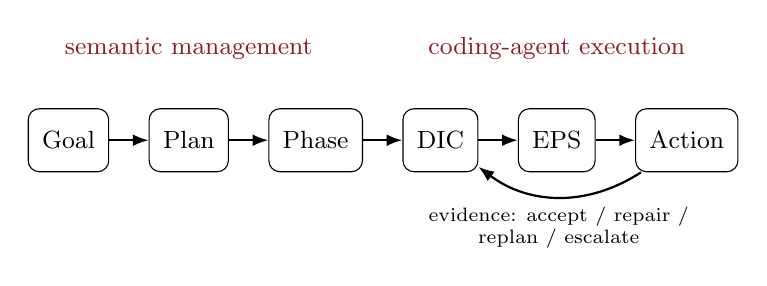
\begin{tikzpicture}[node distance=4mm and 5mm, every node/.style={font=\small}, box/.style={draw,rounded corners,inner sep=5pt,minimum height=8mm}, arr/.style={-{Latex[length=2mm]},thick}]
\node[box] (goal) {Goal};
\node[box,right=of goal] (plan) {Plan};
\node[box,right=of plan] (phase) {Phase};
\node[box,right=of phase] (dic) {DIC};
\node[box,right=of dic] (eps) {EPS};
\node[box,right=of eps] (act) {Action};
\draw[arr] (goal)--(plan);\draw[arr] (plan)--(phase);\draw[arr] (phase)--(dic);\draw[arr] (dic)--(eps);\draw[arr] (eps)--(act);
\node[above=5mm of plan,accent] {semantic management};
\node[above=5mm of eps,accent] {coding-agent execution};
\draw[arr,bend left=35] (act) to node[below,font=\scriptsize,align=center]{evidence: accept / repair /\\ replan / escalate} (dic);
\end{tikzpicture}
\caption{Durable semantic refinement and disposable execution. Replan travels upward; local repair regenerates EPS under the same DIC.}
\label{fig:hierarchy}
\end{figure}

Main is the persistent user-facing semantic manager: it owns Plan authority, one whole-Phase DIC, specialist reconciliation, material decisions, and publication/closure. Theory and Experiment are optional specialist reasoning workstreams; Research is advisory evidence returning to Main. Main also authors the initial EPS/prompt graph for the Phase. Operational execution is delegated to a distinct repository-aware coding-agent \textbf{Orchestrator}, which validates that EPS, compiles its prompt wording for the actual model/surface, routes bounded Workers/subagents, manages safe parallelism and write ownership, integrates returns, performs contract-preserving repair through superseding EPS revisions, and dispatches verification. Routine execution should remain below the human-attention boundary unless scientific meaning or decisive evidence changes.

\subsection{Human-attention objective}
Let $A_H$ be recorded human supervisory attention (measured duration when available, otherwise intervention counts by class) and let $P_V=\sum_v q_v z_v$ be prespecified weighted progress over evidence-accepted milestones. We define human-attention intensity
\[
\rho_H=\frac{A_H}{P_V+\varepsilon}.
\]
The workflow targets lower $\rho_H$ by moving routine routing, state reconstruction, local repair, and evidence bookkeeping into durable machine-managed surfaces. This is a benchmark-relative objective, not a universal productivity score or an established empirical gain. Human judgement remains mandatory for material scientific, authority, release, and external-action decisions.

\subsection{State and recovery}
A small canonical index, \texttt{.ai-workflow/STATE.json}, stores the active Plan, phase summaries, checkpoints, escalations, roles, and evidence pointers. Multi-view DIC packages, EPS prompt/run instantiations, Action records, and mandatory flat Phase reports are stored beneath the Plan/Phase path and linked by identifiers and hashes. A fresh context can reconstruct the approved objective, current phase, lineage, and unresolved governance events from the package alone. Narrative handoffs are views rather than competing authorities.

\subsection{Verification loop}
Verification consumes the DIC, state, and evidence and returns
$\{\mathsf{accept},\mathsf{repair},\mathsf{replan},\mathsf{escalate}\}$.
Repair preserves the DIC and regenerates EPS. Replan changes the decomposition, acceptance meaning, or protocol. Escalation is immediate for material objective, authority, scientific-claim, protocol, destructive/external, release/submission, paid-compute, or credential changes. Routine local failures remain machine decisions.

\section{Formal analysis}
\subsection{Refinement and composition}
Associate every hierarchy object $X$ with admitted traces $\llbracket X\rrbracket$. For an abstraction map $\rho$, define $X\preceq Y$ when $\rho(\llbracket X\rrbracket)\subseteq\llbracket Y\rrbracket$. Refinement chains preserve the parent intent only when the maps compose and each inclusion is sound; hierarchy does not establish those facts automatically.

For a Plan DAG, let each phase implement a sound pre/post contract, let predecessor postconditions imply successor preconditions, require noninterference for unordered writes, and let terminal postconditions imply the global goal. Standard induction over a topological order then yields compositional satisfaction. This identifies the real assumptions hidden by informal ``manager decomposes task'' descriptions.

\subsection{Dependency-local recovery}
Let phase $v$ declare read keys $R_v$ and write keys $W_v$; dependency edges include every possible data flow. If a repair changes keys $\Delta$, define
\[
B(\Delta)=\{v:R_v\cap\Delta\ne\varnothing\},\qquad
\mathcal I(\Delta)=\Reach(B(\Delta)).
\]
\begin{theorem}[Local recovery]
If phase outputs and evidence depend only on declared inputs, tool/version parameters, predecessor outputs, and recorded randomness; dependencies are complete; and evidence is version-bound, then retaining completed outputs outside $\mathcal I(\Delta)$ preserves their contract validity.
\end{theorem}
\begin{proof}[Proof sketch]
Outside the cone, a node neither reads a changed key nor depends on a changed predecessor. Topological induction preserves every declared input and therefore its output/evidence validity. Full proof is in the technical report.
\end{proof}
The cone is worst-case tight: choose a direct reader to copy a changed bit and each descendant to propagate it. Every reachable node can then become invalid. This is an agent-workflow adaptation of dependency-graph and incremental-build locality, not a claim that those underlying ideas are new \citep{mokhov2018build}.

\subsection{Imperfect verification and checkpoints}
If the conditional probability of missing a persisting observable fault at each gate is at most $\alpha<1$, survival through $k$ gates is at most $\alpha^k$, and expected detection delay is at most $1/(1-\alpha)$ gate intervals. In a stationary model with checkpoint cost $c_v$, false-rejection probability $\beta$ and cost $c_f$, fault rate $\lambda$, and per-phase repair cost $c_r$, expected overhead at interval $h$ is
\[
U(h)=\frac{n(c_v+\beta c_f)}h+\lambda n c_r h\frac{1+\alpha}{2(1-\alpha)},
\]
with continuous minimizer
$h^*=\sqrt{2(c_v+\beta c_f)(1-\alpha)/(\lambda c_r(1+\alpha))}$.
This motivates configurable checkpoints rather than per-phase human approval or a universal fixed cadence \citep{young1974first,daly2006higher}.

\subsection{Observability limit}
If evidence map $O$ assigns the same observation to states $s_+$ and $s_-$ while the goal is true only at $s_+$, every evidence-only verifier makes the same decision on both and therefore incurs a false acceptance or false rejection. Hierarchy cannot recover information absent from the evidence channel.

\section{Reference implementation}
The v5.6.39 standard-library runtime implements atomic state updates, Plan/Phase creation, exactly one three-view DIC per Phase, DIC graph validation, Main-authored initial EPS plus disposable repair attempts, Action lineage, the four verification outcomes, package recovery, and prompt-tuning gates. Model-executed EPS nodes must record their actual model profile, execution surface, and applicable prompt-guidance profile before an Action can be recorded. The conformance matrix in \cref{tab:tests} covers structural and governance behavior; it is not comparative agent-performance evidence.
\begin{table}[t]
\centering\small
\begin{tabularx}{\linewidth}{@{}X l@{}}
\toprule
Property & Validation artifact\\\midrule
One Plan authorizes several phases & unit test\\
Ordinary phase progression without approval ceremony & unit test\\
Periodic checkpoint trigger & unit test\\
Immediate material escalation & unit test\\
Action$\to$EPS$\to$DIC$\to$Phase$\to$Plan lineage & unit test + recovery audit\\
Main/Theory/Experiment ownership and aliases & unit test\\
Fresh-session package recovery & unit test + CLI audit\\
Reasonable v5.6.31 compatibility & migration-index test\\
\bottomrule
\end{tabularx}
\caption{Engineering conformance coverage. The release checklist resolves actual build logs; these are not comparative agent results.}
\label{tab:tests}
\end{table}

A deterministic structural fixture changes one declared key in a seven-node workflow. The impact cone contains four nodes rather than all seven, demonstrating that the implementation computes the intended invalidation scope. The fixture assumes complete declarations and does not establish that language models will produce them reliably.

\section{Evaluation programme}
The central question is whether hierarchy's relative benefit increases with effective task horizon. We vary dependency depth, branching, delayed dependencies, interacting constraints, and hidden intermediate faults across objectively graded repository, pipeline, and evidence-synthesis tasks.

The main conditions are C0 direct/reactive; C1 flat plan-and-execute; C2 contracted hierarchy; and C3 hierarchy plus verification-triggered repair/replanning. C1+V spends C3's verifier calls on generic critique without local invalidation; C2-extra spends the same budget on additional generation. These controls distinguish the mechanism from extra tokens, calls, stronger prompts, and verifier-as-inference.

Primary outcomes are end-to-end success, hard-constraint satisfaction, unsupported completion, fault-detection latency, propagation size, recovery locality, and rework; costs include calls, tokens, tools, and wall time. The primary analysis tests a condition-by-effective-horizon interaction with matched task instances and mixed effects. A positive paper claim requires frozen prompts and graders, matched-budget analysis, at least two task families, and all primary conditions. Current unit/smoke evidence does not cross this gate.

\section{Related work and positioning}
Planning/search methods organize within-task reasoning \citep{yao2023react,yao2023tot,besta2024got,prasad2024adapt,zhou2024lats}; compound-agent systems organize roles and conversations \citep{li2023camel,wu2023autogen,chen2024agentverse,hong2024metagpt}; memory systems externalize context \citep{packer2023memgpt,wang2024hiagent}; and workflow optimizers search prompts or agent graphs \citep{khattab2024dspy,hu2025adas}. Our protocol is complementary: it makes authority, semantic refinement, evidence, invalidation, and human checkpoints persistent and inspectable across executions.

AgentBench, WebArena, GAIA, SWE-bench, OSWorld, and $\tau$-bench document hard stateful tasks \citep{liu2024agentbench,zhou2024webarena,mialon2024gaia,jimenez2024swebench,xie2024osworld,yao2024taubench}. We propose controlled graph/fault manipulation because benchmark score alone does not identify why a hierarchy helps. Scalable oversight and process supervision motivate verification but do not make verifiers sound \citep{lightman2023verify,irving2018debate,leike2018recursive}.

\section{Limitations and responsible use}
The mechanism adds overhead on short tasks. DICs can also shift rather than reduce human burden when they are verbose, poorly prioritized, or require frequent reconstruction; salience and compactness are therefore part of the interface contract. DICs and dependency footprints can be wrong, hidden state invalidates local recovery, and verifier errors may be correlated. Role separation does not guarantee independent judgment. The runtime is not a security boundary; prompt injection, malicious tools, and mutable external services require separate controls \citep{ruan2024toolemu,debenedetti2024agentdojo}. The formal cost model is stylized; human-attention intensity uses task-specific progress weights and imperfect proxies for cognitive effort; and no confirmatory performance or attention-efficiency result is claimed.

\paragraph{Responsible-use statement.} The system is intended to make agent authority, evidence, and intervention points more visible, not to authorize unsupervised high-impact actions. Deployments should minimize credentials and external permissions, sandbox tools, preserve audit logs, require explicit human approval for destructive, release, submission, financial, privacy-sensitive, or other high-impact actions, and test for prompt injection and evidence manipulation. The workflow may create a false sense of assurance when contracts or verifiers are weak; users should treat residual uncertainty as part of the output.

\section{Conclusion}
A useful meta-agent needs more than another planning prompt. It needs a durable object that says what remains authoritative, which objective is primary, how intent was refined, what evidence supports progress, what a repair invalidates, and when human attention is actually required. Contracted hierarchies provide that object while separating a persistent semantic manager from repository-aware coding-agent orchestration. The implementation and theory establish a defensible mechanism and its limits; the frozen matched-budget study is the next gate for any claim that the system improves trustworthy long-horizon progress or lowers human attention required per unit of verified progress.

\bibliographystyle{plainnat}
\bibliography{references}
\end{document}
